%% Copernicus Publications Manuscript Preparation Template for LaTeX Submissions
%% ---------------------------------
%% This template should be used for copernicus.cls
%% The class file and some style files are bundled in the Copernicus Latex Package which can be downloaded from the different journal webpages.
%% For further assistance please contact the Copernicus Publications at: publications@copernicus.org
%% http://publications.copernicus.org


%% Please use the following documentclass and Journal Abbreviations for Discussion Papers and Final Revised Papers.


%% 2-Column Papers and Discussion Papers
\documentclass[gmd, manuscript]{copernicus}



%% Journal Abbreviations (Please use the same for Discussion Papers and Final Revised Papers)

% Archives Animal Breeding (aab)
% Atmospheric Chemistry and Physics (acp)
% Advances in Geosciences (adgeo)
% Advances in Statistical Climatology, Meteorology and Oceanography (ascmo)
% Annales Geophysicae (angeo)
% ASTRA Proceedings (ap)
% Atmospheric Measurement Techniques (amt)
% Advances in Radio Science (ars)
% Advances in Science and Research (asr)
% Biogeosciences (bg)
% Climate of the Past (cp)
% Drinking Water Engineering and Science (dwes)
% Earth System Dynamics (esd)
% Earth Surface Dynamics (esurf)
% Earth System Science Data (essd)
% Fossil Record (fr)
% Geographica Helvetica (gh)
% Geoscientific Instrumentation, Methods and Data Systems (gi)
% Geoscientific Model Development (gmd)
% Geothermal Energy Science (gtes)
% Hydrology and Earth System Sciences (hess)
% History of Geo- and Space Sciences (hgss)
% Journal of Sensors and Sensor Systems (jsss)
% Mechanical Sciences (ms)
% Natural Hazards and Earth System Sciences (nhess)
% Nonlinear Processes in Geophysics (npg)
% Ocean Science (os)
% Proceedings of the International Association of Hydrological Sciences (piahs)
% Primate Biology (pb)
% Scientific Drilling (sd)
% SOIL (soil)
% Solid Earth (se)
% The Cryosphere (tc)
% Web Ecology (we)



%% \usepackage commands included in the copernicus.cls:
%\usepackage[german, english]{babel}
%\usepackage{tabularx}
%\usepackage{cancel}
%\usepackage{multirow}
%\usepackage{supertabular}
%\usepackage{algorithmic}
%\usepackage{algorithm}
%\usepackage{float}
%\usepackage{subfig}
%\usepackage{rotating}

% cmz - Additional added packages
%\usepackage{rotating}
%\usepackage{color}


\begin{document}

%\nolinenumbers
\linenumbers

\title{Impact of ocean coupling strategy on extremes in high-resolution atmospheric simulations}


% \Author[affil]{given_name}{surname}

\Author[1]{Colin M.}{Zarzycki}
\Author[2]{Kevin A.}{Reed}
\Author[1]{Julio}{Bacmeister}
\Author[1]{Susan C.}{Bates}
\Author[1]{Anthony P.}{Craig}
\Author[1]{Nan A.}{Rosenbloom}

\affil[1]{Climate and Global Dynamics, National Center for Atmospheric Research, Boulder, Colorado, USA.}
\affil[2]{School of Marine and Atmospheric Sciences, State University of New York at Stony Brook, Stony Brook, New York, USA.}

%% The [] brackets identify the author with the corresponding affiliation. 1, 2, 3, etc. should be inserted.

\runningtitle{OCEAN COUPLING IMPACT ON CLIMATE EXTREMES}

\runningauthor{ZARZYCKI ET AL.}

\correspondence{Colin M. Zarzycki, Climate and Global Dynamics, National Center for Atmospheric Research, Boulder, Colorado, USA. (zarzycki@ucar.edu)}

\received{}
\pubdiscuss{} %% only important for two-stage journals
\revised{}
\accepted{}
\published{}

%% These dates will be inserted by Copernicus Publications during the typesetting process.

\firstpage{1}

\maketitle

\begin{abstract}

This paper discusses the sensitivity of tropical cyclone climatology to ocean coupling strategy in high-resolution configurations of the Community Earth System Model. Using two supported model setups, we demonstrate that the choice of grid on which the lowest model level wind stress and surface fluxes are computed may lead to differences in cyclone strength in multi-decadal climate simulations, particularly for the most intense cyclones. Using a deterministic framework, we show that when these surface quantities are calculated on an ocean grid that is coarser than the atmosphere, the computed frictional stress is misaligned with wind vectors in individual atmospheric grid cells. This reduces the effective surface drag, and results in more intense cyclones when compared to a model configuration where the ocean and atmosphere are of equivalent resolution. Our results demonstrate that the choice of computation grid for atmosphere/ocean interactions is non-negligible when considering climate extremes at high horizontal resolution, especially when model components are on highly disparate grids.

\end{abstract}

\introduction  %% \introduction[modified heading if necessary]
The use of general circulation models (GCMs) to evaluate global tropical cyclone (TC) characteristics in current and future climate has grown considerably over the last decade.  It has been shown that GCMs can model TCs at horizontal resolutions of approximately 100 km grid spacing, albeit with limitations \citep[e.g.,][]{Bengtsson2007a,Knutson2010,Strachan2013}. As GCMs have advanced to even higher horizontal resolutions (i.e., $\le 50$ km) the simulated climatology of tropical cyclones has improved greatly \citep[e.g.,][]{Oouchi2006,Zhao2009,Murakami2012,Manganello2012,Satoh2012,Bacmeister2014,Wehner2014,Reed2015}. Furthermore, the use of variable-resolution GCMs has shown to be useful for the study of regional TC climatologies at reduced computational cost compared to equivalent global high-resolution simulations, providing further resources capable of pushing climate simulations to finer grid spacings \citep{Zarzycki2014,Zarzycki2014AMIPTCs}.  

Recently, intercomparisons have shown that the range of simulated TC climatology across different climate models can be large \citep{Camargo2013CMIP,Walsh2015CLIVAR}.  It has also been shown that, within individual GCMs, TC characteristics can vary greatly depending on model design choices. Various studies have documented the large uncertainty in TC simulations due to the choice of individual subgrid parameterizations, such as cumulus parameterizations \citep[e.g.,][]{Kim2012,Reed2011CAMPhysics,Lim2014TCconv}), while others have focused on differences due to changes in whole parameterization suites \citep{Reed2011c,Bacmeister2014}. The dynamical core, the main fluid flow component of a GCM, has also been shown to be an important source of uncertainty for TC simulations, though less widely documented \citep{ReedSimplePhys,Zhao2012,Reed2015}.

In this manuscript we describe another mechanism through which simulated TC properties are influenced by model design choices, in particular, the manner in which the ocean and atmosphere are coupled within the climate system. Specifically, we will utilize the Community Atmosphere Model version 5 (CAM5), within the Community Earth System Model (CESM), to explore the impact of two different strategies for coupling to a prescribed ocean. CAM5 has shown increasing ability to model tropical cyclones at high horizontal resolutions of 0.25\degree{} \citep{Bacmeister2014,Zarzycki2014AMIPTCs,Wehner2014,Wehner2015,Reed2015} and a similar model setup will be used for part of this study.

The remainder of the paper is organized as follows. Section \ref{sec:model} provides an introduction to the modeling system used in this study and how coupling between the atmosphere and ocean is treated. Section \ref{sec:climate} investigates the impact on multi-year climate simulations while Section \ref{sec:forecast} details the sensitivity of TCs to the ocean grid using a deterministic forecast framework. Section \ref{sec:discussion} discusses the results and offers further insight into their implications.

%------------------------------------------------

\section{Model description}
\label{sec:model}

\subsection{Community Earth System Model}
\label{subsec:cam}

In this paper, we utilize CESM, which is a community climate model allowing for atmospheric simulations to be coupled to land, ocean, and ice models \citep{Hurrell2013CESM}. The atmospheric component, CAM5 \citep{CAM5Tech}, is configured with the Spectral Element (SE) dynamical core. SE is the newest dynamical core available in CAM5 and is based upon continuous Galerkin spectral finite elements which are applied on a cubed-sphere grid \citep{Taylor1997,Thomas2005,Taylor2010}. In addition to attractive conservation characteristics \citep{Taylor2011}, CAM-SE has shown appealing scaling properties since atmospheric primitive equations are solved locally on individual elements \citep{Dennis2012,Evans2013}. The land model is the Community Land Model (CLM) version 4.0 run in satellite phenology (SP) mode \citep{CLM40Tech}. While CESM also allows for coupling to dynamic ocean and ice models, all of the simulations here utilize prescribed sea surface temperatures (SSTs) and ice cover concentrations. Using data forcing for the ocean and ice models is a commonly-used configuration to minimize the computational cost associated with high-resolution atmospheric modeling \citep{Walsh2015CLIVAR}. In the default CESM configuration, prescribed SSTs and ice are passed to the model on a 1\degree{}x1\degree{} grid and internally interpolated to the particular ocean and ice grids.

\subsection{Coupling within CESM}
\label{subsec:coupling}

When all earth system model components operate on identical grids, vertical coupling (such as between the ocean surface and lowest level of the atmosphere) is straightforward. However, since  components are generally not integrated on the same spatial grid, CPL7 is used to couple these components to one another within the CESM framework \citep{Craig2012}. The coupler utilizes remapping weights to regrid quantities which are needed across model components. Figure \ref{fig:coupling-schematic} provides a schematic of the standard coupling process when differences exist between, for example, the resolution of the atmosphere and ocean grids in CESM. In this case, the atmospheric grid (red) is of finer resolution. As smaller atmospheric grid spacings become more common in simulations utilizing prescribed SSTs and ice data forcing, it's no longer typical for the ocean resolution to be similar or finer in resolution in such setups. Therefore, having the atmospheric grid be the finest in the climate system is the default setup for many high-resolution configurations in CESM. 

Atmospheric variables, such as winds (black vectors; taken here to approximate the flow associated with a Northern Hemisphere tropical cyclone), are computed on the atmospheric grid (Fig. \ref{fig:coupling-schematic}a). Generally, CESM has computed atmosphere/ocean fluxes on the ocean grid. Therefore, when coupling is required, these values are then conservatively remapped to the ocean grid (blue) (Fig. \ref{fig:coupling-schematic}b). Surface momentum stress ($\tau$, gray vectors) and sensible and latent heat fluxes are calculated on the ocean grid using these remapped values (Fig. \ref{fig:coupling-schematic}c). The calculated quantities are then remapped back to the atmospheric grid using either conservative remapping or bilinear interpolation (Fig. \ref{fig:coupling-schematic}d), where they are used by the atmospheric component of the model for integration (Fig. \ref{fig:coupling-schematic}e). While the exact techniques that various GCMs use to couple model components are not identical, this general framework of mapping required quantities across grids is commonly used.

\begin{figure}
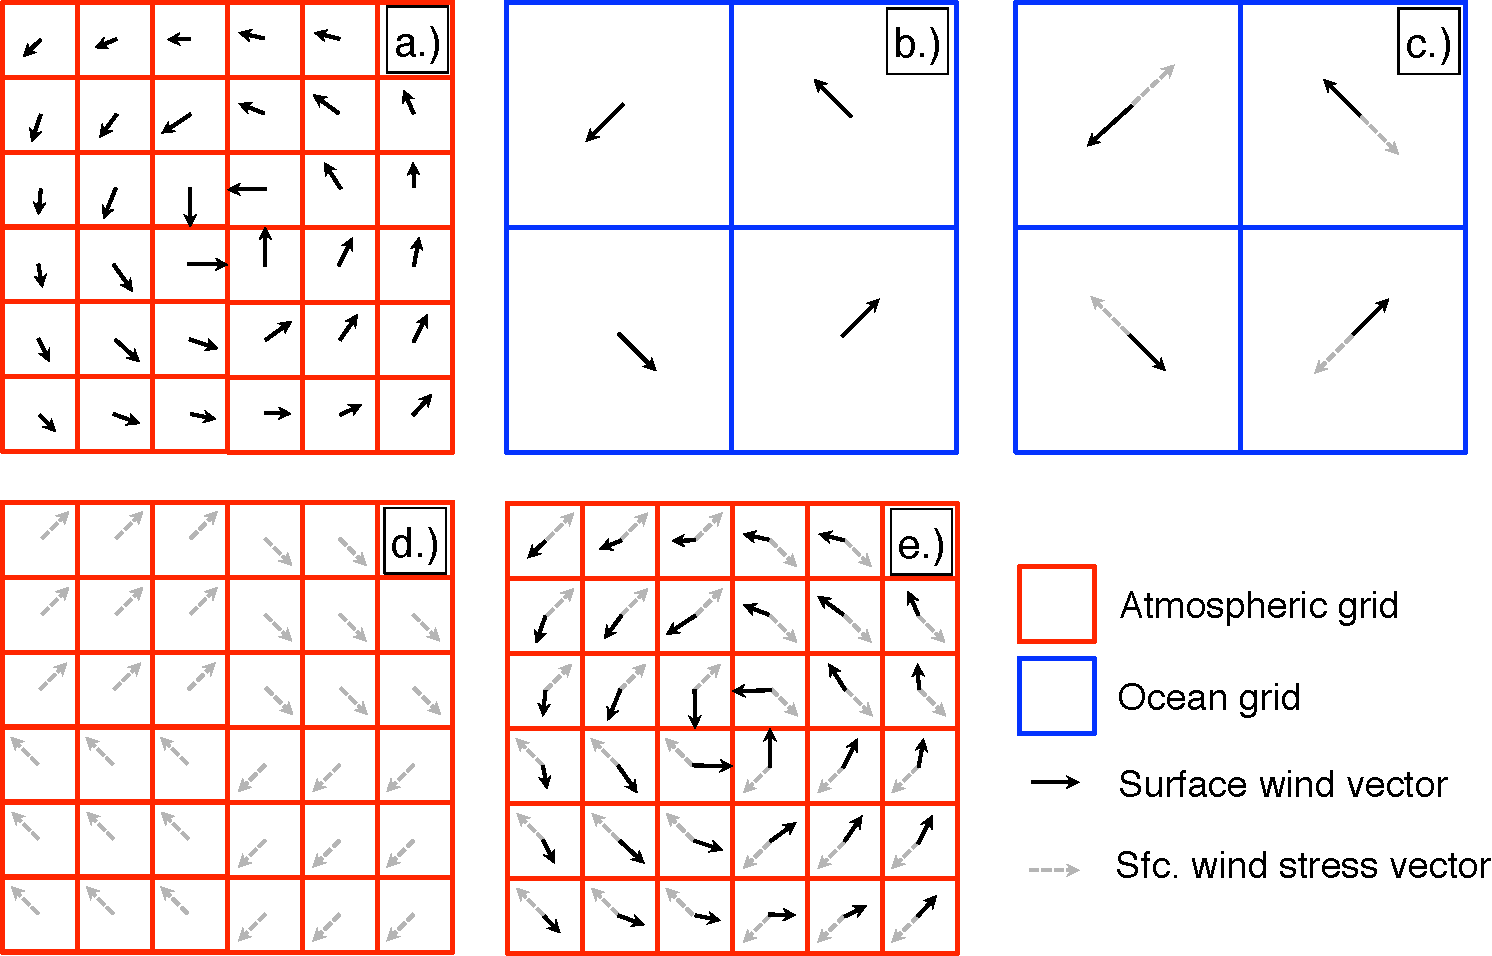
\includegraphics[width=0.85\linewidth]{fig_coupling-schematic.pdf}
\caption{Coupling procedure in CESM. Red (blue) boxes indicate atmospheric (ocean) grid cells. Black (Gray) solid (dashed) vectors show surface wind (wind stress) vectors.}
\label{fig:coupling-schematic}
\end{figure}

\section{Climate simulations}
\label{sec:climate}

We first compare TC statistics in two multi-decadal climate simulations using 0.25\degree{} (\textasciitilde{}28 km, denoted as ne120 on the spectral element cubed sphere grid) resolution for the atmosphere. Both simulations follow Atmospheric Model Intercomparison Project (AMIP) protocols \citep{Gates1992} and are coupled to CLM on a standard latitude-longitude grid with an equivalent  resolution of approximately 0.25\degree{}. The first simulation is coupled to a prescribed ocean/ice model on a grid where the polar point is displaced over Greenland, which is at approximately 1\degree{} horizontal resolution (ne120\_gx1v6). This is coarser than both the atmosphere and land models. The second simulation is identical to the first, except the prescribed ocean/ice model operates on the same 0.25\degree{} (ne120) grid as the atmosphere and land (ne120\_ne120). For both simulations, all atmosphere/ocean coupling calculations are carried out on the ocean grid. We note that these are both supported, `out of the box,' grid configurations in CESM. SSTs and ice coverage are applied using the monthly 1\degree{} Hadley Centre Sea Ice and Sea Surface Temperature dataset (HadISST, \citet{Hurrell2008}). While the ocean/ice model may operate on the 0.25\degree{} grid, all data is interpolated from the same 1\degree{} dataset. Therefore, the higher resolution ocean grid does not provide more spatial structure in surface forcing, isolating the effect of solely the resolution of the coupling calculations.

Both simulations are integrated from 1980 to 2005. Taylor statistics for the 1980-2000 global-mean quantities for sea-level pressure (PSL), total precipitable water (TMQ), total precipitation rate (PRECT), 200 hPa zonal wind (U200), 850 hPa zonal wind (U850), 600 hPa relative humidity (RH600) and 500 hPa temperature (T500) are shown in Fig. \ref{fig:taylor_global}. The two simulations are compared to observational datasets including NCEP \citep{Kalnay1996} (PSL, U200, U850, RH600, T500), MERRA \citep{Rienecker2011} (TMQ), and TRMM \citep{TRMM3B43} (PRECT). The absolute distance from the origin (lower left) represents the magnitude of the spatial variability within the domain (as measured by normalized standard deviation) while the spatial correlation is plotted as the radial angle between the model marker and the origin. A comprehensive discussion of Taylor diagram analysis can be found in \citet{Taylor2001}. Red dots highlight the climatology of the ne120\_ne120 simulation while blue dots show the same for the ne120\_gx1v6 simulation. This analysis is only concerned with the relative difference between the two simulations and, therefore, whether or not mean climatology is impacted by choice of coupling grid. A thorough analysis to understand why each parameter is modeled with their particular skill in CAM5 itself is beyond the scope of this paper. We do note, however, that the results are consistent with skill scores reported in previous CAM5 modeling studies, such as \citet{Bacmeister2014} (their Figs. 2 and 3) and \citet{Zarzycki2015AMIP} (their Fig. 9).

\begin{figure}
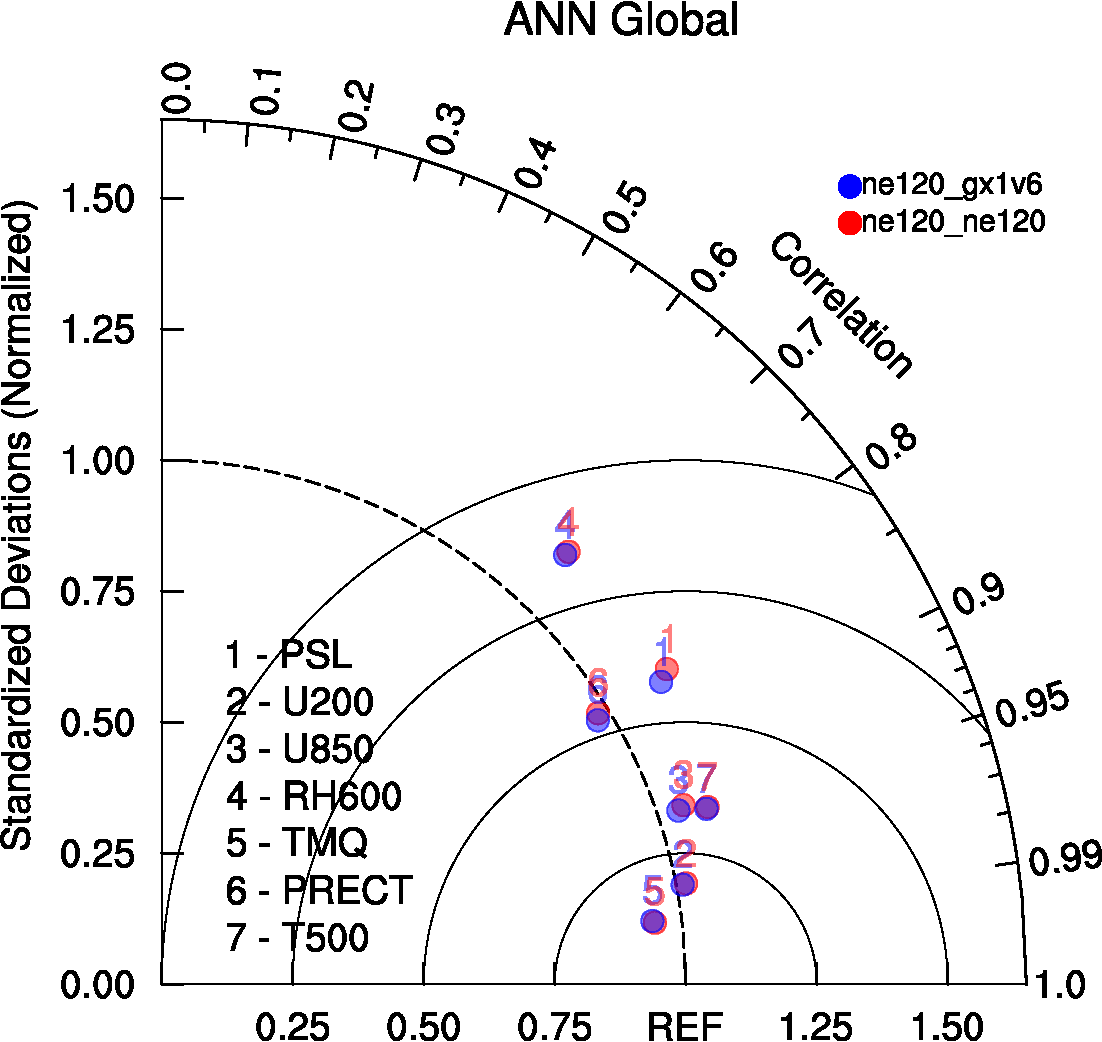
\includegraphics[width=0.6\linewidth]{fig_taylor_globe_ANN.pdf}
\caption{Taylor diagram for globally- and annually-averaged climate statistics. Blue circles represent the results from AMIP simulation coupled to 1\degree{} ocean grid (ne120\_gx1v6) and red circles represent the same for simulation using 0.25\degree{} ocean grid (ne120\_ne120). See text for description of the diagram and explanation of acronyms.}
\label{fig:taylor_global}
\end{figure}

The most notable result from assessing this skill is the two simulations are highly similar in a global climatological sense. All markers representing the ne120\_gx1v6 simulation overlap with their corresponding variable from the ne120\_ne120 simulation. The occurrence of this overlap highlights that the mean climate state is not impacted by choice of coupling strategy in the climate simulations.

However, while the mean climatologies of the two simulations are essentially identical, notable differences arise when comparing TC statistics between the two simulations. TCs are objectively tracked in model output using the method first outlined in \citet{Vitart1997} and updated by \citet{Knutson2007}. The version of the TC tracker applied in this study utilizes 3-hourly model output from the atmospheric component and is described in detail in \citet{Zhao2009}. Previous work using this technique to find TCs in CAM/CESM output have produced a reasonable storm climatology both spatially and in terms of storm intensity \citep{Reed2015}. For the tracker, all data is regridded from the CAM-SE ne120 cubed sphere grid to a 0.25\degree{} latitude-longitude grid as in \citet{Reed2015}. Surface winds (taken to be at a height of 10 m) are approximated from the lowermost model level winds ($\approx$ 60 m) and a logarithmic law as described in \citet{Zarzycki2014AMIPTCs}.

\begin{table}
\caption{Annual frequency of global tropical cyclones that reach tropical storm (cat. 0-5), hurricane (cat. 1-5) and major hurricane (cat. 4-5) strength the CAM5 simulations and IBTrACS observations for the time period of 1980 to 2005.}\label{tc_counts}
\begin{tabular}{l c c c}
\hline
\textbf{Simulation} & \textbf{Total Storms} & \textbf{Hurricanes} & \textbf{Major Hurricanes}\\
\hline
IBTrACS         & 91.6 $\pm$ 8.5    & 47.1 $\pm$ 5.5 & 10.7 $\pm$ 3.3 \\
ne120$\_$gx1v6 &  70.1 $\pm$ 9.0   & 55.5 $\pm$ 7.7  & 12.5 $\pm$ 3.4\\
ne120$\_$ne120 & 73.2 $\pm$ 10.5  & 50.3 $\pm$ 8.2 & 4.2   $\pm$ 1.9 \\
\hline
\end{tabular}
\end{table}

Table~\ref{tc_counts} displays storm counts for all TCs, storms that reach hurricane strength (\textgreater 33 m s$^{-1}$) and storms that reach major hurricane strength (\textgreater 59 m s$^{-1}$) on the Saffir-Simpson scale \citep{Simpson1974} (major hurricane defined here as categories 4 and 5) for each simulation for 1980 through 2005. Observations from the International Best Track Archive for Climate Stewardship (IBTrACS, \citet{Knapp2010}) for the same time period are provided as a reference. Both simulations produce roughly the same frequency of total storms, with the ne120\_ne120 configuration only producing approximately 4$\%$ more TCs annually.  However, despite this, the simulation coupled to the lower resolution ocean (ne120\_gx1v6) produces 10$\%$ more hurricanes and nearly three times the amount of major hurricanes when compared to the simulation with the higher resolution coupling. Given that the total number of storms is roughly equivalent between the two configurations, this signifies a shift in the overall intensity distribution towards stronger TCs in the ne120\_gx1v6 setup.

To explore this further, Figure~\ref{fig:preswind} displays the minimum surface pressure versus maximum 10-m wind speed relationship for TCs in each simulation with a quadratic least squares fit shown as a solid line. IBTrACS observations are again included as a reference. To be consistent with the TC tracker, only storms that reach tropical storm strength in their lifetime are used. At low wind speeds (i.e., \textless 40 m s$^{-1}$) the relationship between the minimum surface pressure and maximum wind speed for the two model simulations and observations compare well.  However, at larger wind speeds the relationship between the two simulations diverges consistent to the differences in TC counts in Table~\ref{tc_counts}. In particular, the ne120$\_$gx1v6 simulation produces greater winds speeds at a given minimum pressure than the ne120$\_$ne120 simulation, suggesting the ocean coupling resolution impact on tropical cyclone intensity is non-negligible, especially with respect to intense TCs.

\begin{figure}
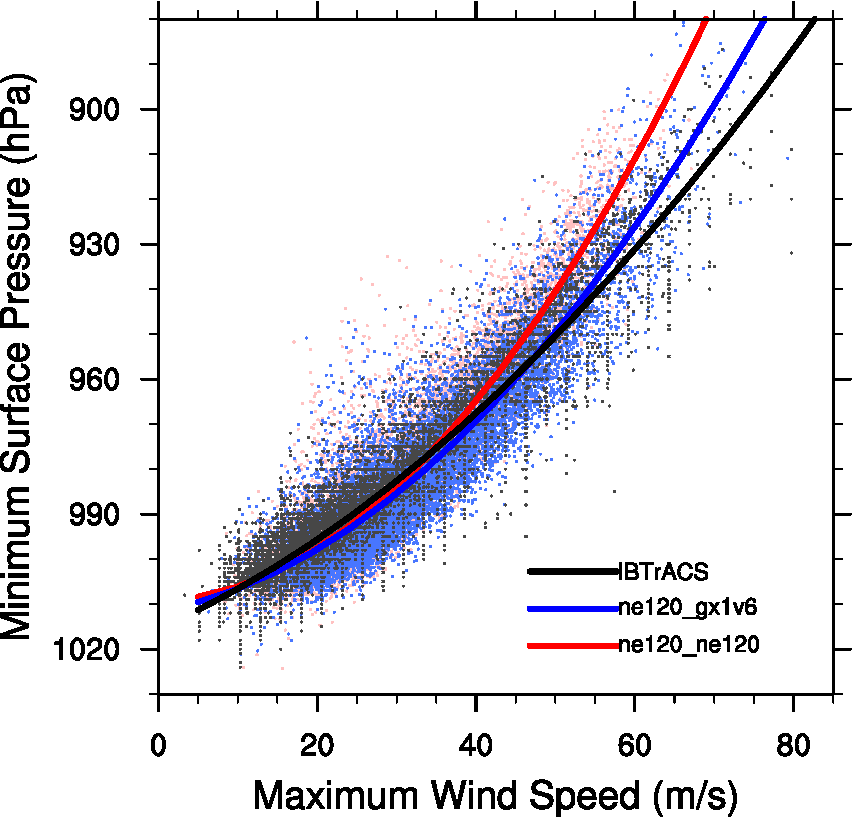
\includegraphics[width=0.6\linewidth]{fig_preswind.pdf}
\caption{Storm minimum surface pressure vs. maximum 10-m wind speed relationship with quadratic least squares fit (solid lines) for the CAM5 simulations and IBTrACS observations from 1980 to 2005. Note that 3-hourly output is used for the model simulations, while the IBTrACS data is 6-hourly.}
\label{fig:preswind}
\end{figure}

Figure \ref{fig:wind-pdfs} shows the number of annual 10-m TC wind exceedances in the 3-hourly model output for both category 3 and category 4 storm thresholds. These represent two of the most intense classifications of tropical cyclones, with maximum 10-m winds surpassing 50 m s$^{-1}$ and 59 m s$^{-1}$, respectively. The blue curve with open markers indicates the number of 3-hour samples within the TC trajectories which surpass each threshold in the simulation using the 1\degree{} ocean/ice grid (ne120\_gx1v6). The red curve with filled markers represents the same for the simulation with the 0.25\degree{} ocean/ice grid (ne120\_ne120). From the left panel, we see that for all years (except 1985 and 1988), the simulation coupled to the coarser ocean grid produces a significantly greater frequency of category 3 level winds, with the average number of annual instances being approximately 6 times higher than when using the high-resolution ocean grid. This behavior is even more pronounced in the right panel, where the ne120\_gx1v6 simulation averages approximately 10 instances of category 4 level winds per year. However, this threshold is not exceeded at any point during the 25-year sample in the ne120\_ne120 simulation.

\begin{figure}
\begin{tabular}{c c}
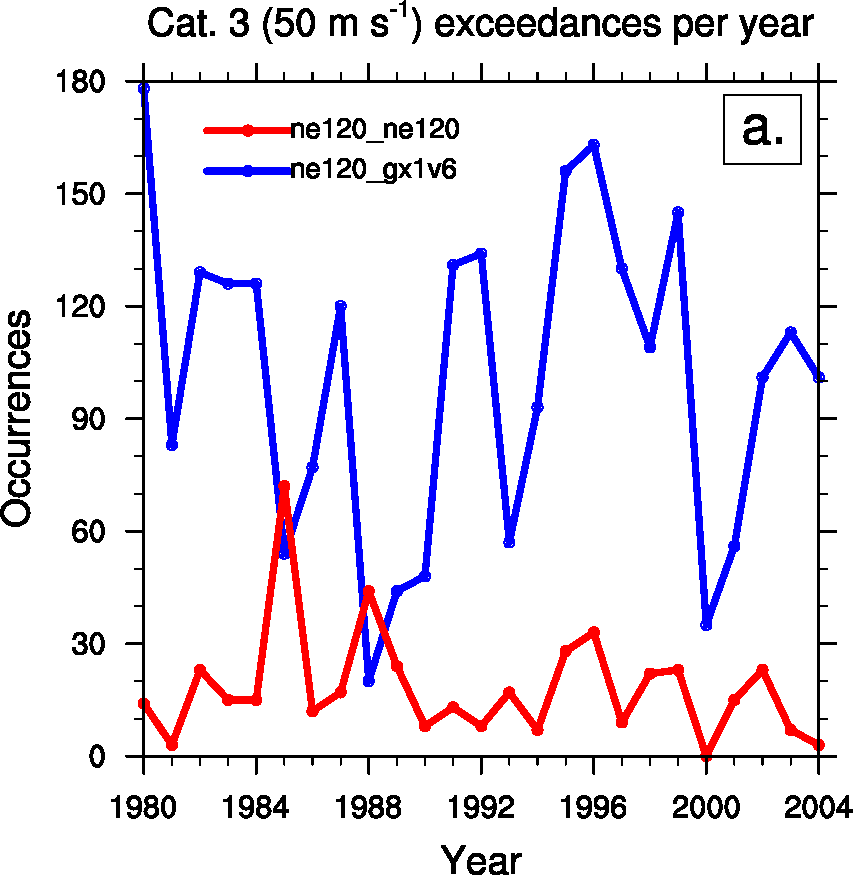
\includegraphics[width=0.405\linewidth]{fig_u10exceed_cat3.pdf} & 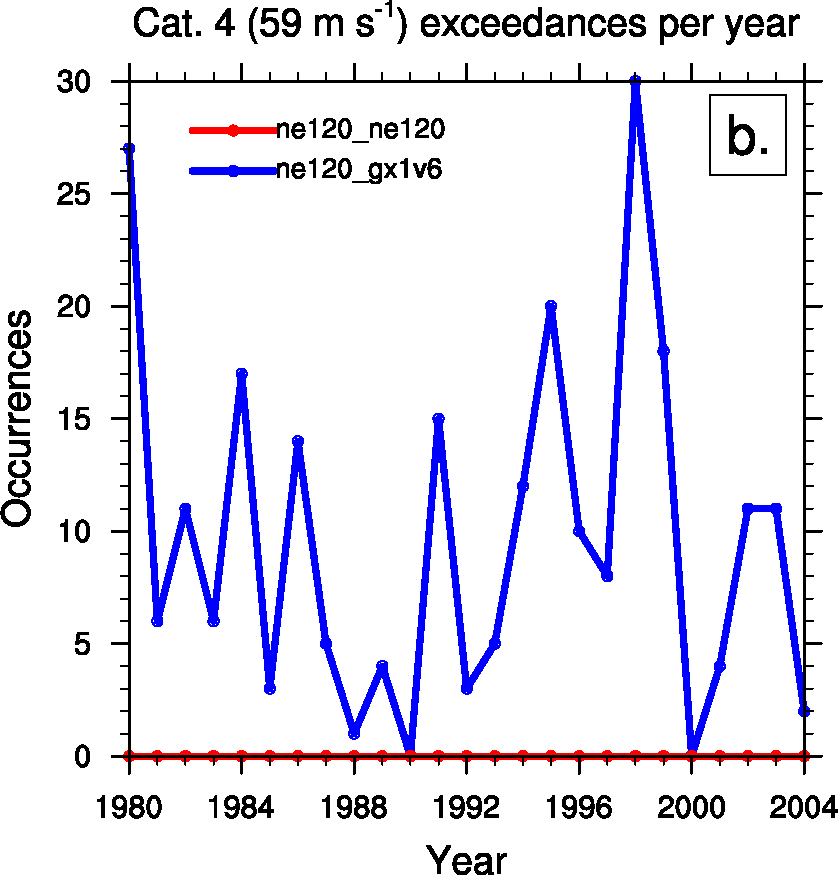
\includegraphics[width=0.4\linewidth]{fig_u10exceed_cat4.pdf}
\end{tabular}
\caption{Number of TC surface wind instances exceeding category 3 and category 4 wind thresholds for AMIP simulation coupled to 1\degree{} ocean grid (ne120\_gx1v6) and 0.25\degree{} ocean grid (ne120\_ne120). Instances are calculated using 3-hourly TC trajectories.}
\label{fig:wind-pdfs}
\end{figure}


%------------------------------------------------

\section{Deterministic simulations}
\label{sec:forecast}

Since all aspects of the model configurations in Section \ref{sec:climate} are identical except for the grid on which the prescribed SSTs and ice concentrations are passed to the other model components (and therefore the atmosphere/ocean exchange computation grid), we hypothesize that the marked difference in TC climatology is induced by the coupling strategy and difference in grid resolutions. To assess the differences in simulated TCs in a controlled, deterministic manner, we utilize two identical CAM setups to complete short-term forecast simulations of observed storms. These simulations utilize the new, variable-resolution capability of CAM-SE \citep{Zarzycki2014APE}.

The setup is similar to that used in the previous section, but the model is configured with a variable-resolution atmospheric grid with 0.125\degree{} (\textasciitilde{}14 km, ne240) resolution over the Atlantic Ocean. Forecast simulations are initialized with a digitally-filtered atmospheric analysis from the National Centers for Environmental Predictions (NCEP) Global Data Assimilation System (GDAS). Observed SSTs on a 1\degree{}x1\degree{} grid are derived from the NOAA High-resolution Blended Analysis \citep{Reynolds2007}. The land surface is modeled by CLM 4.0 and is initialized with a state nudged to be in balance with the atmospheric initial conditions. The model setup and initialization are both thoroughly detailed in \citet{Zarzycki2015TCForecast}.

As in the climate simulations, the only difference between the two setups is the grid used by the data ocean and ice models. The first set of simulations uses the aforementioned displaced pole grid with an equivalent resolution of 1\degree{} (ne240\_gx1v6) while the second uses an ocean grid identical to the atmospheric grid with an equivalent resolution of 0.125\degree{} (ne240\_ne240). Since the SST and ice cover data are provided at coarser scales than the model interpolates to, any differences in the results again arise due to the differences in calculating of surface fluxes and momentum drag on the corresponding ocean grids.

After initialization, each configuration is integrated for 8 days. Figure \ref{fig:forecast_panels} shows the 120-hour forecasts for Hurricane Leslie in the North Atlantic Ocean from the 2012 hurricane season. The simulation was initialized at 00Z on August 31st, 2012, making Fig. \ref{fig:forecast_panels} valid at 00Z on September 5th, 2012. The forecast using the 1\degree{} ocean grid is on the left (Fig. \ref{fig:forecast_panels}a,d), with the 0.125\degree{} ocean grid in the center (Fig. \ref{fig:forecast_panels}b,e). In Figs. \ref{fig:forecast_panels}a,b,d,e all calculations are done on the ocean grid. All fields are extracted from the atmospheric model component.

The top panels depict instantaneous lowest model level wind (black vectors) as well as the surface frictional stress vector (red). In Fig. \ref{fig:forecast_panels}a, it is readily apparent that many instances exist where the vectors are not aligned. This results from the surface stress being calculated on the coarser ocean grid. This coarser information is then used to provide stress information at the higher resolution used by the atmospheric numerics (as in Fig. \ref{fig:coupling-schematic}). In Fig. \ref{fig:forecast_panels}b, the wind and stress vectors are parallel (180\degree{} difference), indicating that the frictional drag is acting in direct opposition to the wind within the atmospheric dynamical core, which is the expected behavior from theory. The higher resolution ocean grid preserves the resolution of the surface wind field during stress calculations. Because of this, not only are the stress vectors properly aligned with the high-resolution ocean grid, the maximum magnitudes of the stress vectors are larger at the storm's radius of maximum wind in Fig. \ref{fig:forecast_panels}b when compared against Fig. \ref{fig:forecast_panels}a.

This highlights that maxima in the stress field at the atmospheric grid cell scale are conserved with the higher resolution ocean grid, whereas these maxima are ``smoothed'' in the calculation where wind is first averaged to the coarser ocean grid (Fig. \ref{fig:forecast_panels}a). This is further evidenced by the fact that the integrated dot product (over a 3\degree{}x3\degree{} domain centered over the TC minimum surface pressure) of the two fields is approximately 20\% smaller in the simulations using the 1\degree{} ocean grid. Therefore, the use of the coarser ocean grid results in a misaligned, and therefore universally weaker, frictional force fed back to the atmospheric dynamics, leading to enhanced extreme wind speeds.

\begin{figure}
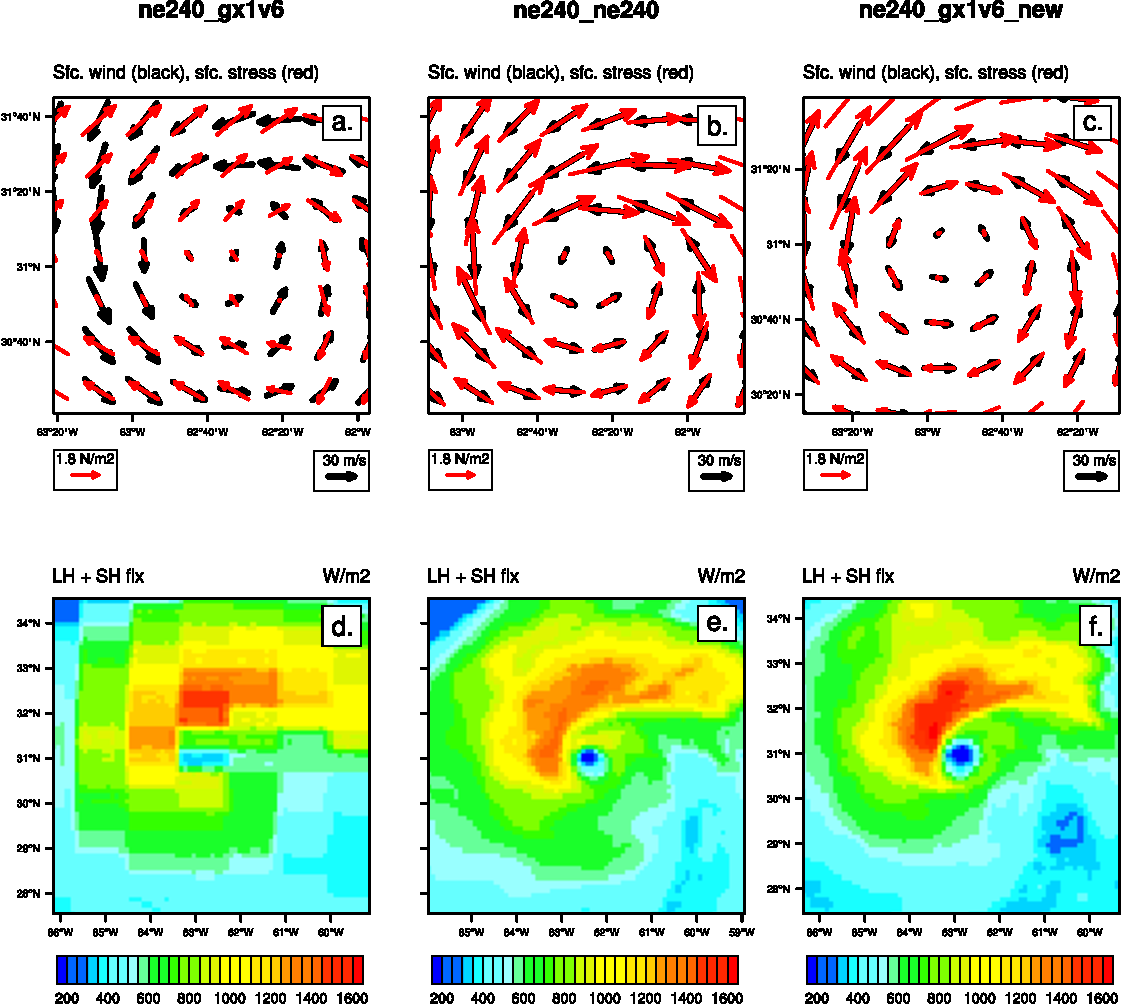
\includegraphics[width=0.85\linewidth]{fig_compareStress.pdf}
\caption{120-hour CAM-SE forecast for Hurricane Leslie, valid at 00Z on September 5th, 2012. Left panels (a,d) are results from forecast using 1\degree{} ocean grid in the default configuration (calculations carried out on ocean grid). Center panels (b,e) show results using 0.125\degree{} ocean grid. Right panels show version of 1\degree{} grid where calculations are carried out on the atmospheric grid. Top panels (a-c) display instantaneous wind in the lowest model (black vectors) with corresponding lowest model level wind stress (red vectors). Lower panels (d-f) show total surface flux (latent plus sensible heat).}
\label{fig:forecast_panels}
\end{figure}

The cumulative surface heat (sensible plus latent) flux is shown on the bottom of Fig. \ref{fig:forecast_panels} for the two storms at the same forecast time. It is clear that the coarser ocean grid (Fig. \ref{fig:forecast_panels}d) provides information back to the atmosphere with significantly less spatial structure than the 0.125\degree{} ocean grid (Fig. \ref{fig:forecast_panels}e). While the difference in 5\degree{}x5\degree{} integrated heat flux is relatively small (approximately 1\%), it is clear that the spatial structure of the heat flux field is very different between the two model configurations. This may further play a role in storm dynamics, with the 1\degree{} ocean grid providing a larger, more diffuse source of surface heating to the TC core than the high-resolution grid.

To conclusively verify that this discrepancy arises from the choice of coupling, we complete a third simulation, which is identical to the ne240\_gx1v6 simulation, except coupling calculations are carried out on the higher-resolution atmospheric grid (ne240\_gx1v6\_reverse) instead of the ocean. If the TC behavior in the ne240\_gx1v6 configuration is due to errors arising from carrying out computations on the coarser grid in the coupling system, we expect this to be primarily alleviated by ensuring coupling is carried out on the higher-resolution grid. This should result in maximum spatial resolution of the computed fields and no `loss' of information due to interpolation from fine to coarse and back to fine resolutions. Figures \ref{fig:forecast_panels}c,f show the same analysis as with the previous configurations. It is obvious that inverting the grid to ensure calculations of surface stresses and fluxes are done on the higher resolution grid (in this case, the atmosphere) results in a solution that looks much more similar to the configuration where both atmosphere and ocean are of high resolution (Figs. \ref{fig:forecast_panels}b,e). We note that these two simulations (ne240\_ne240 and ne240\_gx1v6\_reverse) are not fully identical due to the fact that remapping is still required in the ne240\_gx1v6\_reverse calculations. Examples of prominent similarities include the fact that surface stresses are stronger and aligned parallel to lowest model level wind vectors and that there is additional fine scale structure in the total surface flux field.

\conclusions
\label{sec:discussion}

This manuscript describes biases in atmospheric extreme climatology which arise from choice of ocean grid and coupling strategy in CESM. Since surface stress and flux calculations are carried out on the ocean grid, running the model with a coarser ocean than atmosphere presents problems with respect to tropical cyclone (TC) climatology. In particular, surface stress vectors which are passed back to the atmospheric dynamical core following coupling are not aligned with the surface wind due to being computed on a coarser grid. This allows winds near the core of TCs to become stronger than if the stresses were computed at the same resolution of the atmosphere. Additionally, when surface fluxes are calculated on a coarser grid, the influxes of heat and moisture to the lowest levels of the atmosphere underneath the TC are structurally different, with these quantities being more diffuse and misaligned with the maximum surface wind, in contradiction to bulk aerodynamic flux theory.

The issues outlined in the manuscript underscore that the choice of ocean grid when using SST and ice data to force a dynamic atmosphere is not trivial, even if the native resolution of this forcing data is  relatively coarse. However, they are easy to correct for these configurations, particularly since applying coupled atmosphere-ocean calculations on the same grid is straightforward and computationally inexpensive.

More problematic adjustments may arise when coupling to a dynamical ocean model. The vast majority of coupled, dynamic simulations not only utilize differing resolutions between different model components, but also different numerical techniques and grids. Therefore, remapping between components is, in many cases, an absolute necessity. The obvious recommendation to alleviate coupling inconsistencies when it is not feasible to use identical grids is to calculate these quantities on the finest resolution grid of the coupled system. Performing coupling in this manner ensures that information passed back to a model component has not been interpolated to a resolution coarser than the component's native resolution during the coupling process. In addition, in integrated models which allow for multiple grid options, the choice of the model component defining the grid for these calculations should not be pre-configured for all cases, but rather, determined dynamically based on the various resolutions chosen for the particular model setup.

However, we emphasize that, even when applying this suggestion, it is not clear that it is fully appropriate for coupled dynamical models to be run at highly disparate resolutions from one another, where processes interacting between components may be sufficiently non-linear that essentially averaging from a higher resolution grid is not the most appropriate mechanism. Further work will be required to determine whether or not this is the case. Additionally, this strategy is not elementary when variable-resolution grids are coupled to uniform grids, particularly where the finest and coarsest scales of the multi-resolution grid may straddle the grid scales of the uniform-resolution component. In these cases, the choice of `finer' grid in the atmosphere-ocean coupling will be different depending on the region of interest, and may require even more flexible frameworks, such as exchange grids \citep{Balaji2006,Valcke2012coupling}.

Our results demonstrate that the mean climatology of the simulations presented here are essentially identical regardless of coupling strategy, highlighting that this impact only becomes readily apparent in the tail of the distributions of interest. However, with climate models being used more and more frequently for direct analysis of extreme events, including TCs, both in present climate and under future scenarios, this sensitivity of model-derived extremes may become more prevalent.  This is especially relevant as atmospheric models continue to march forward with respect to horizontal resolution, and therefore, their ability to dynamically resolve phenomena at smaller and smaller spatial scales. Consideration of these impacts when utilizing high-resolution climate data for analysis is required and modifications to how the current generation of atmospheric models treats coupling between various earth system components in supported configurations may be necessary.



\begin{acknowledgements}
The National Center for Atmospheric Research is sponsored by the National Science Foundation. The authors would like to thank John E. Truesdale for assistance in performing the simulations. Resources of the Argonne Leadership Computing Facility at Argonne National Laboratory, which is supported by the Office of Science of the U.S. Department of Energy under contract DE-AC02-06CH11357, were used for this research. Furthermore, this work utilizes part of the "Using Petascale Computing Capabilities to Address Climate Change Uncertainties" PRAC allocation support by the National Science Foundation ACI-1036146. This work is also part of the Blue Waters sustained-petascale computing project, which is supported by the National Science Foundation (awards OCI-0725070 and ACI-1238993) and the state of Illinois. Blue Waters is a joint effort of the University of Illinois at Urbana-Champaign and its National Center for Supercomputing Applications. Bacmeister was partially supported through the Scientific Discovery through Advanced Computing (SciDAC) program funded by U.S. Department of Energy, Office of Science, Advanced Scientific Computing Research. Bates was supported by the Regional and Global Climate Modeling Program (RGCM) of the US. Department of Energy, Office of Science (BER), Cooperative Agreement DE-FC02-97ER62402. IBTrACS data were freely obtained from the National Oceanic and Atmospheric Administration (http://www.ncdc.noaa.gov/ibtracs/). Model data from all simulations in this manuscript are archived and available at NCAR upon request through the authors.
\end{acknowledgements}


%% REFERENCES

%% The reference list is compiled as follows:

%% Since the Copernicus LaTeX package includes the BibTeX style file copernicus.bst,
%% authors experienced with BibTeX only have to include the following two lines:
%%
\bibliographystyle{copernicus}
\bibliography{references.bib}
%%
%% URLs and DOIs can be entered in your BibTeX file as:
%%
%% URL = {http://www.xyz.org/~jones/idx_g.htm}
%% DOI = {10.5194/xyz}


%% LITERATURE CITATIONS
%%
%% command                        & example result
%% \citet{jones90}|               & Jones et al. (1990)
%% \citep{jones90}|               & (Jones et al., 1990)
%% \citep{jones90,jones93}|       & (Jones et al., 1990, 1993)
%% \citep[p.~32]{jones90}|        & (Jones et al., 1990, p.~32)
%% \citep[e.g.,][]{jones90}|      & (e.g., Jones et al., 1990)
%% \citep[e.g.,][p.~32]{jones90}| & (e.g., Jones et al., 1990, p.~32)
%% \citeauthor{jones90}|          & Jones et al.
%% \citeyear{jones90}|            & 1990



%% FIGURES

%% ONE-COLUMN FIGURES

%%f
%\begin{figure}[t]
%\includegraphics[width=8.3cm]{FILE NAME}
%\caption{TEXT}
%\end{figure}
%
%%% TWO-COLUMN FIGURES
%
%%f
%\begin{figure*}[t]
%\includegraphics[width=12cm]{FILE NAME}
%\caption{TEXT}
%\end{figure*}
%
%
%%% TABLES
%%%
%%% The different columns must be seperated with a & command and should
%%% end with \\ to identify the column brake.
%
%%% ONE-COLUMN TABLE
%
%%t
%\begin{table}[t]
%\caption{TEXT}
%\begin{tabular}{column = lcr}
%\tophline
%
%\middlehline
%
%\bottomhline
%\end{tabular}
%\belowtable{} % Table Footnotes
%\end{table}
%
%%% TWO-COLUMN TABLE
%
%%t
%\begin{table*}[t]
%\caption{TEXT}
%\begin{tabular}{column = lcr}
%\tophline
%
%\middlehline
%
%\bottomhline
%\end{tabular}
%\belowtable{} % Table Footnotes
%\end{table*}
%
%
%%% NUMBERING OF FIGURES AND TABLES
%%%
%%% If figures and tables must be numbered 1a, 1b, etc. the following command
%%% should be inserted before the begin{} command.
%
%\addtocounter{figure}{-1}\renewcommand{\thefigure}{\arabic{figure}a}
%
%
%%% MATHEMATICAL EXPRESSIONS
%
%%% All papers typeset by Copernicus Publications follow the math typesetting regulations
%%% given by the IUPAC Green Book (IUPAC: Quantities, Units and Symbols in Physical Chemistry,
%%% 2nd Edn., Blackwell Science, available at: http://old.iupac.org/publications/books/gbook/green_book_2ed.pdf, 1993).
%%%
%%% Physical quantities/variables are typeset in italic font (t for time, T for Temperature)
%%% Indices which are not defined are typeset in italic font (x, y, z, a, b, c)
%%% Items/objects which are defined are typeset in roman font (Car A, Car B)
%%% Descriptions/specifications which are defined by itself are typeset in roman font (abs, rel, ref, tot, net, ice)
%%% Abbreviations from 2 letters are typeset in roman font (RH, LAI)
%%% Vectors are identified in bold italic font using \vec{x}
%%% Matrices are identified in bold roman font
%%% Multiplication signs are typeset using the LaTeX commands \times (for vector products, grids, and exponential notations) or \cdot
%%% The character * should not be applied as mutliplication sign
%
%
%%% EQUATIONS
%
%%% Single-row equation
%
%\begin{equation}
%
%\end{equation}
%
%%% Multiline equation
%
%\begin{align}
%& 3 + 5 = 8\\
%& 3 + 5 = 8\\
%& 3 + 5 = 8
%\end{align}
%
%
%%% MATRICES
%
%\begin{matrix}
%x & y & z\\
%x & y & z\\
%x & y & z\\
%\end{matrix}
%
%
%%% ALGORITHM
%
%\begin{algorithm}
%\caption{�}
%\label{a1}
%\begin{algorithmic}
%�
%\end{algorithmic}
%\end{algorithm}
%
%
%%% CHEMICAL FORMULAS AND REACTIONS
%
%%% For formulas embedded in the text, please use \chem{}
%
%%% The reaction environment creates labels including the letter R, i.e. (R1), (R2), etc.
%
%\begin{reaction}
%%% \rightarrow should be used for normal (one-way) chemical reactions
%%% \rightleftharpoons should be used for equilibria
%%% \leftrightarrow should be used for resonance structures
%\end{reaction}
%
%
%%% PHYSICAL UNITS
%%%
%%% Please use \unit{} and apply the exponential notation


\end{document}
